\documentclass[11pt,a4paper]{article}
\usepackage[margin=2.5cm]{geometry}
\usepackage{booktabs}
\usepackage{listings}
\usepackage{xcolor}
\usepackage{graphicx}
\usepackage{float}

\lstset{
  basicstyle=\ttfamily\small,
  frame=single,
  backgroundcolor=\color{gray!8},
  breaklines=true
}

\title{Labwork 6: Map}
\author{Yanis Denizot -- 2640051}
\date{\today}

\begin{document}
\maketitle

\section{Implementation}
The three labworks are map operations: each output pixel only depends on the input pixel at
the same position. So all the kernels have the same structure as the 2D grayscale kernel of
labwork 4: each thread computes its \texttt{x} and \texttt{y}, checks that it is inside the
image, and processes one pixel. I ran everything on Google Colab (Tesla T4) with a
$1200 \times 800$ image.

\textbf{6a: Binarization.} I first convert the image to grayscale with one value per pixel,
then each pixel becomes white (255) if it is above the threshold, or black (0). I use 255
instead of 1 so the result can be displayed. The threshold is 128.
\begin{lstlisting}[language=Python]
if src[y, x] >= threshold:
    dst[y, x] = 255
else:
    dst[y, x] = 0
\end{lstlisting}

\textbf{6b: Brightness control.} I add a value \texttt{delta} to the 3 channels (positive to
increase, negative to decrease). The result must stay between 0 and 255, otherwise the
\texttt{uint8} value overflows and bright pixels become dark.
\begin{lstlisting}[language=Python]
for c in range(3):
    v = src[y, x, c] + delta
    if v > 255:
        v = 255
    if v < 0:
        v = 0
    dst[y, x, c] = v
\end{lstlisting}

\textbf{6c: Blending.} The output is $Q = c \cdot I_1 + (1 - c) \cdot I_2$ for each channel.
The two images must have the same size, so for $I_2$ I used the same photo flipped
horizontally, with $c = 0.5$.
\begin{lstlisting}[language=Python]
for c in range(3):
    dst[y, x, c] = np.uint8(coef * src1[y, x, c] + (1 - coef) * src2[y, x, c])
\end{lstlisting}

\begin{figure}[H]
\centering
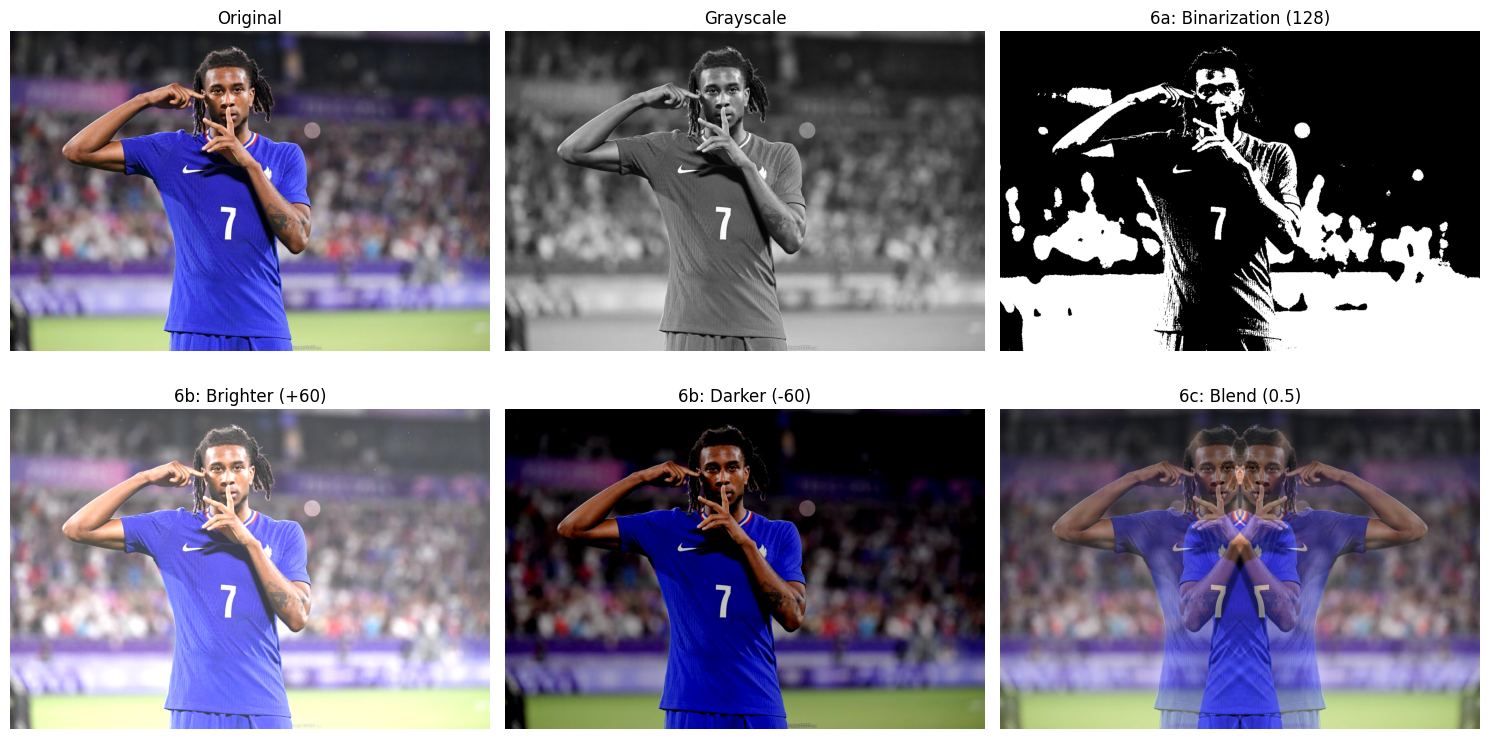
\includegraphics[width=\textwidth]{results.png}
\end{figure}

\section{Block size}
Each time is the average of 100 launches.

\begin{table}[H]
\centering
\begin{tabular}{lrrr}
\toprule
Block & Binarization ($\mu$s) & Brightness ($\mu$s) & Blending ($\mu$s) \\
\midrule
$8 \times 8$   & 64.1 & 94.1 & 382.9 \\
$16 \times 8$  & 36.4 & 64.3 & 382.5 \\
$16 \times 16$ & 33.5 & 68.6 & 381.3 \\
$32 \times 16$ & 41.6 & 65.6 & 390.0 \\
$32 \times 32$ & 42.6 & 80.6 & 395.4 \\
\bottomrule
\end{tabular}
\end{table}

\begin{figure}[H]
\centering
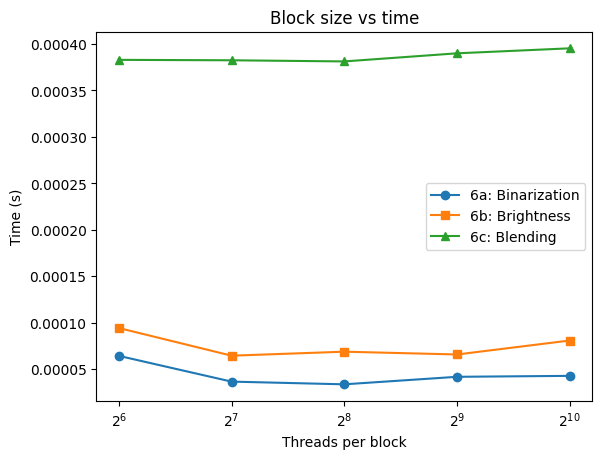
\includegraphics[width=0.65\textwidth]{blocksize_vs_time.png}
\end{figure}

These kernels do almost no computation, so the time mostly depends on the memory read and
written. Binarization is the fastest because it reads and writes only 1 value per pixel,
while brightness uses 3 values (R, G, B). The $8 \times 8$ blocks are the slowest, because a
warp covers 4 small parts of different rows, so the memory accesses are less grouped. The
best sizes are around $16 \times 8$ and $16 \times 16$, and $32 \times 32$ is a bit slower
like in the previous labworks.

Blending was much slower than the others (about 6 times slower than brightness), even if it
only reads one more image. The reason is that \texttt{coef} is a Python float, so the
computation is done in double precision (float64), and the T4 is 32 times slower in float64
than in float32 (``FP32/FP64 Performance Ratio: 32'' in labwork 2). I tested a version where
everything is converted to \texttt{np.float32}:

\begin{table}[H]
\centering
\begin{tabular}{lr}
\toprule
Blending ($16 \times 16$) & Time ($\mu$s) \\
\midrule
float64 & 382.3 \\
float32 & 85.2 \\
\bottomrule
\end{tabular}
\end{table}

With float32, blending is 4.5 times faster and close to the brightness kernel, so on this
GPU it is important to avoid float64.

\end{document}
